\chapter{Background and Related Work}\label{ch:background-and-related-work}

While Virtual Reality technology has gained more and more traction over the recent years, 30\% to 80\% of users
encounter some form of sickness symptoms during their exposure to virtual environments~\cite{Rebenitsch2016}.
Additionally, these sickness symptoms can have lasting effects after the exposure as well~\cite{LaViola2000}.
The high number of affected users has led to cybersickness being one of, if not the biggest roadblock to a more
widespread adoption of Virtual Reality Devices.

According to LaViola~\cite{LaViola2000} the symptoms of exposure to virtual environments include:
\begin{itemize}
    \item Eye strain
    \item Headache
    \item Pallor
    \item Sweating
    \item Dryness of mouth
    \item Fullness of stomach
    \item Disorientation
    \item Vertigo
    \item Nausea
    \item Vomiting.
\end{itemize}
Vertigo, in the case of VR-sickness particularly benign paroxysmal positional vertigo (BPPV), is a condition where the
individual experiences a false sense of motion, or spinning, and objects or surroundings appear to swirl or
move~\cite{Post2010}.
\\
Several studies also found that severity of symptoms increases with longer exposure times to virtual environments~\cite{Ruddle2004,Min2004,Duzmanska2018}.
However, some studies show that users can adapt, and overall sickness reduces with repeated exposure~\cite{Hill2000}.

Throughout the study of these symptoms, several terms have been used to compound these sickness symptoms that appear
to be similar to the symptoms of motion sickness.
Initially, the term Simulator Sickness was used to describe motion sickness encountered during exposure to flight
simulators~\cite{Saredakis2020}.
The term originated from the assessment of military flight simulators~\cite{Kennedy1993}.
While Simulator Sickness is still used in recent publications, the terms Cybersickness or VR Sickness are generally used
to differentiate, and closer examine the side effects of virtual environments from simulator
sickness~\cite{Saredakis2020,McCauley1992}.
The term VR Sickness specifically is used in discussions and studies about sickness symptoms involving head-mounted
displays (HMD)~\cite{Kim2018,Cobb1999}.
This terminology is often used interchangeably across literature.
The terms Cybersickness and VR Sickness will be used in this study, as Stanney, Kennedy, and
Drexler~\cite{Stanney1997} argue that, while sickness from virtual environments shares many of the symptoms also
experienced during simulator sickness or motion sickness, the sickness profiles are different.
\begin{center}
    \begin{tabular}{ l l l l l}
        \toprule
        \textbf{ } & \textbf{Simulator sickness} & \textbf{Sea sickness} & \textbf{Space sickness} &
        \textbf{Cybersickness} \\
        \midrule
        Highest rating & Oculomotor & Nauseagenic & Nauseagenic & Disorientation \\
        Middle rating & Nauseagenic & Oculomotor & Disorientation & Nauseagenic \\
        Lowest rating & Disorientation & Disorientation & Oculomotor & Oculomotor \\
        \bottomrule
    \end{tabular}
    \captionof{table}{Related conditions symptom profiles according to Rebenitsch and Owen~\cite{Rebenitsch2016}.}
    \label{tab:symptom-profiles}
\end{center}
According to Rebenitsch and Owen~\cite{Rebenitsch2016} cybersickness and other sickness symptoms similar to motion
sickness are polysymptomatic (many symptoms) and polygenic (different manifestation for individuals) and therefore
complex to understand and describe.
To make the sickness and its symptoms easier to survey and examine, Kennedy et al.~\cite{Kennedy1993} categorize the
symptoms listed above into three categories:
\begin{itemize}
    \item Nauseagenic symptoms (dryness of mouth, fullness of stomach, nausea, etc.)
    \item Oculomotor sypmtoms (eye strain, headache, etc.)
    \item Disorientation symptoms (vertigo, dizziness, etc.)
\end{itemize}
The main arguments for the distinction between simulator sickness and cybersickness are that during cybersickness,
disorientation symptoms rank highest and oculomotor symptoms rank lowest, while simulator sickness and traditional
motion sickness usually have the inverted profile, where disorientation symptoms rank lowest~\cite{Stanney1997}.

Cybersickness can also occur without stimulation to the vestibular system, purely through visual cues, unlike motion
and simulator sickness, where stimulation of the vestibular system is needed, but not visual stimulation~\cite{LaViola2000}.
Additionally, Stanney et al.~\cite{Stanney1997} determined that cybersickness can be up to three times more severe
than simulator sickness.
Saredakis et al.~\cite{Saredakis2020} also note significantly higher average Simulator Sickness Questionnaire scores,
although both mention, the scores and questionnaire were established with a focus on military flight simulators used
by military personnel.
While recently, the Simulator Sickness Questionnaire has been adopted to measure cybersickness in virtual
environments, which might be the reason for the higher average scores~\cite{Saredakis2020}.


\section{Common causes of cybersickness}\label{sec:common-causes-of-cybersickness}

Over the recent years there have been several theories trying to explain the sickness symptoms experienced during
extended exposure to virtual environments, especially since the commercialisation of head-mounded virtual reality
devices.
The most common Theories are the sensory conflict theory and the postural instability theory.
Additionally, there are some theories that try to explain why sickness symptoms occur in virtual environments like the
rest frame theory, and the vergence accommodation conflict theory.


\subsection{Sensory conflict theory}\label{subsec:sensory-conflict-theory}

The generally most accepted, and widespread theory is based on a sensory mismatch either between sensory systems of the
body, or between sensory input and expectation given the perceived environment.
Most commonly, a sensory conflict due to vection (the illusion of self movement while stationary) is argued to be the
main cause of cybersickness~\cite{Weech2018,Keshavarz2019}.
Although, other studies like Palmisano, Mursic, and Kim~\cite{Palmisano2017} suggest, that vection is neither the
sole, nor primary source of sensory conflict.
Sensory conflicts like vection can also occur outside virtual environments, for example when a person is in a
stationary vehicle while an adjacent vehicle begins to move~\cite{LaViola2000}.

\begin{figure}[h]
    \centering
    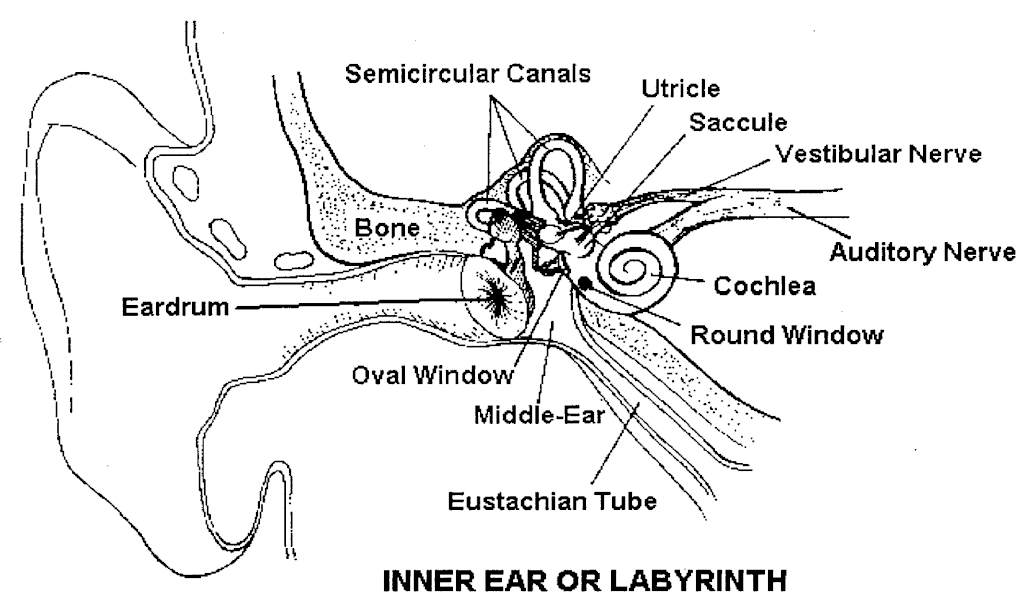
\includegraphics[width=\textwidth]{content/2_related_work/img/VestibularSystem[LaViola2000]}
    \caption{The components of the vestibular system~\cite{LaViola2000}.}
    \label{fig:vestibular-system}
\end{figure}
Important for the sensory conflict theory are visual perception and the vestibular system, shown in
Figure~\ref{fig:vestibular-system}.
The vestibular system consist of the Semicircular Canals to sense angular momentum, and the Utricle and Saccule to
sense linear momentum.
Together, the system functions to compensate for movement, stabilize vision, maintain head posture, and maintain
balance~\cite{Walker2014}.
In virtual environments, the sensory mismatch is usually between the visual system receiving optical flow patterns
characteristic of self motion, while the vestibular system does not perceive these changes in motion.
This sensory conflict lies at the root of simulator sickness and was identified early on, when Barrett and
Thornton~\cite{Barrett1968} noticed that subjects showed simulator sickness symptoms caused by conflict between the
visual presentation of motion and the lack of corresponding vestibular sensation in their fixed-base simulators.
Barrett and Thornton also noticed, that subjects only showed sickness symptoms when the simulator was in a
perspective similar to driving a car, but showed no symptoms when viewing the car from outside, similar to driving a
remote controlled car, as well as passengers showing more severe symptoms than drivers, indicating
that involvement in motion is a factor in the occurrence of simulator sickness~\cite{Tiiro2018,Barrett1968}.

The sensory conflict theory is the most popular theory to explain cybersickness, because it has a steadily growing
amount of studies supporting it, and the theory is intuitive to understand~\cite{Rebenitsch2016,Tiiro2018}.
However, the theory has been criticised by several studies, because sensory conflict theory only states that sickness
is preceded by a sensory conflict, but is unable to predict when cybersickness will occur, or how severe
sickness symptoms will be~\cite{LaViola2000,Rebenitsch2016,Kolasinski1995}.


\subsection{Postural instability theory}\label{subsec:postural-instability-theory}

Another theory for cybersickness symptoms is the postural instability theory proposed by Riccio and Stoffregen~\cite{Riccio1991}.
They found that motion sickness is preceded by periods of postural instability, where small uncontrolled movements and
changes in the subjects centre of gravity occur, and the subject's ability to maintain postural stability is
hindered~\cite{Riccio1991,Clifton2020}.
Stoffregen and Smart~\cite{Stoffregen1998} translated the theory into three predictions:
\begin{itemize}
    \item Experiences of motion sickness are always preceded by increases in postural instability.
    \item Experiences of motion sickness persist until postural stability is restored.
    \item People who are more naturally unstable are more likely to become motion sick during provocative simulation.
\end{itemize}
These predictions have been solidified and are supported by numerous studies on visually induced motion
sickness~\cite{Clifton2020}.
Chardonnet, Mirzaei, and Merienne~\cite{Chardonnet2015}, as well as other studies propose to use the changes in 
range, variance, and frequency of the subject's centre of gravity as a measurement of postural sway.
Based on the accessibility of devices to measure individual's centre of gravity, those measurements have found
increasing popularity in studies to objectively measure subject's postural stability and indicate the potential onset
of cybersickness symptoms~\cite{Lim2020}.
\begin{figure}[h]
    \centering
    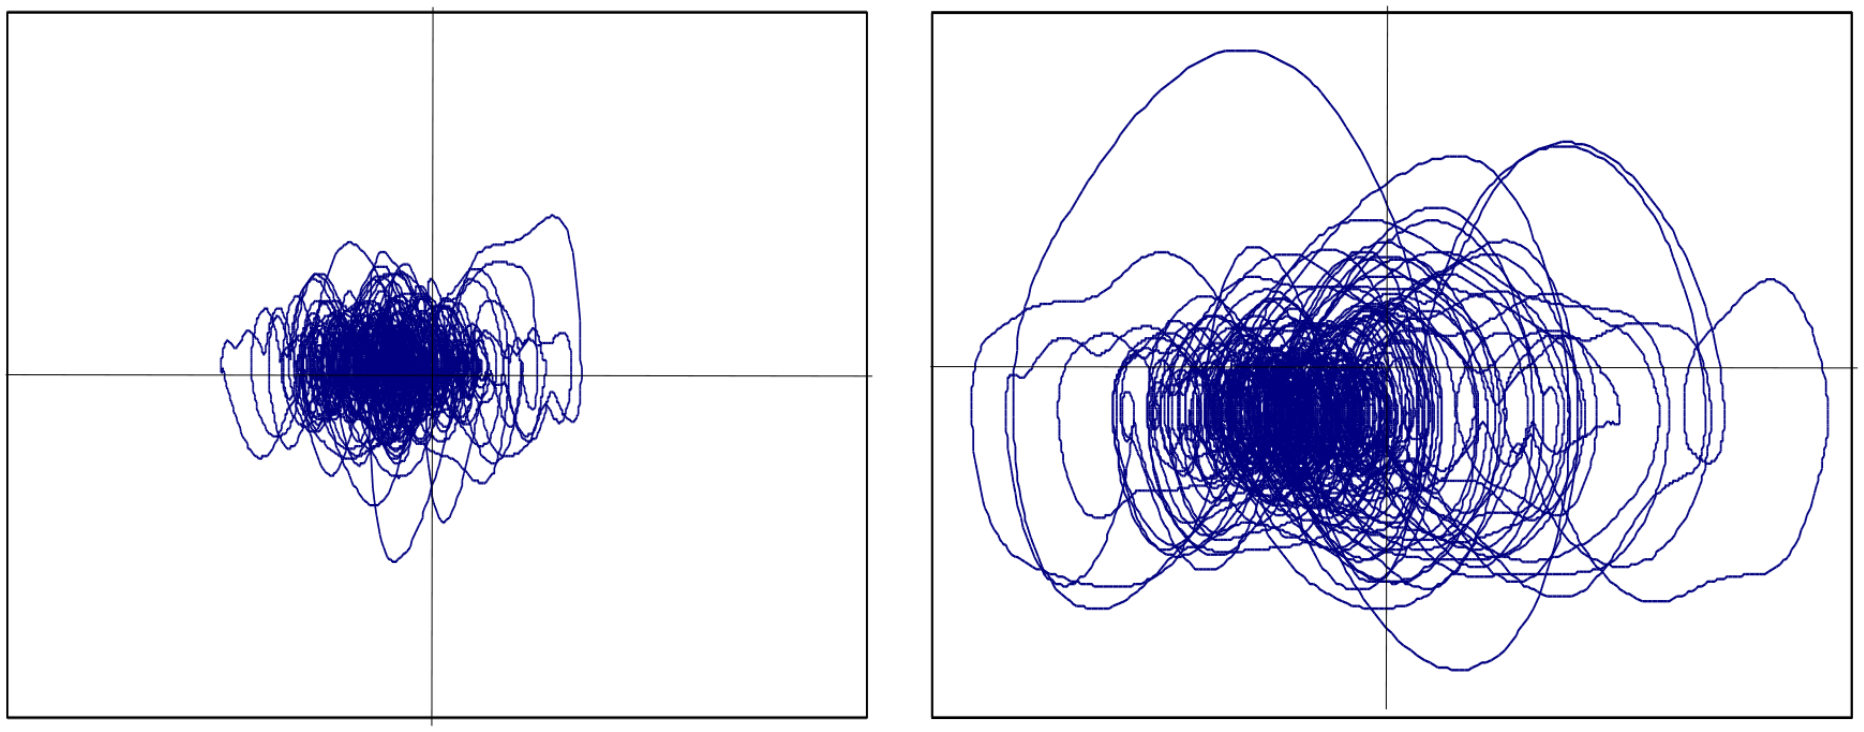
\includegraphics[width=\textwidth]{content/2_related_work/img/PosturalStability[Smart2013]}
    \caption{Comparison of phase portraits (position (in cm) vs. velocity (in cm/s)) for well (left) and sick (right)
        subjects in a dataset measuring postural stability~\cite{Smart2013}.}
    \label{fig:postural-instability-sample}
\end{figure}
A comparison between the natural postural sway of a subject compared to the postural sway when experiencing motion
sickness is shown in Figure~\ref{fig:postural-instability-sample}.
\begin{figure}[h]
    \centering
    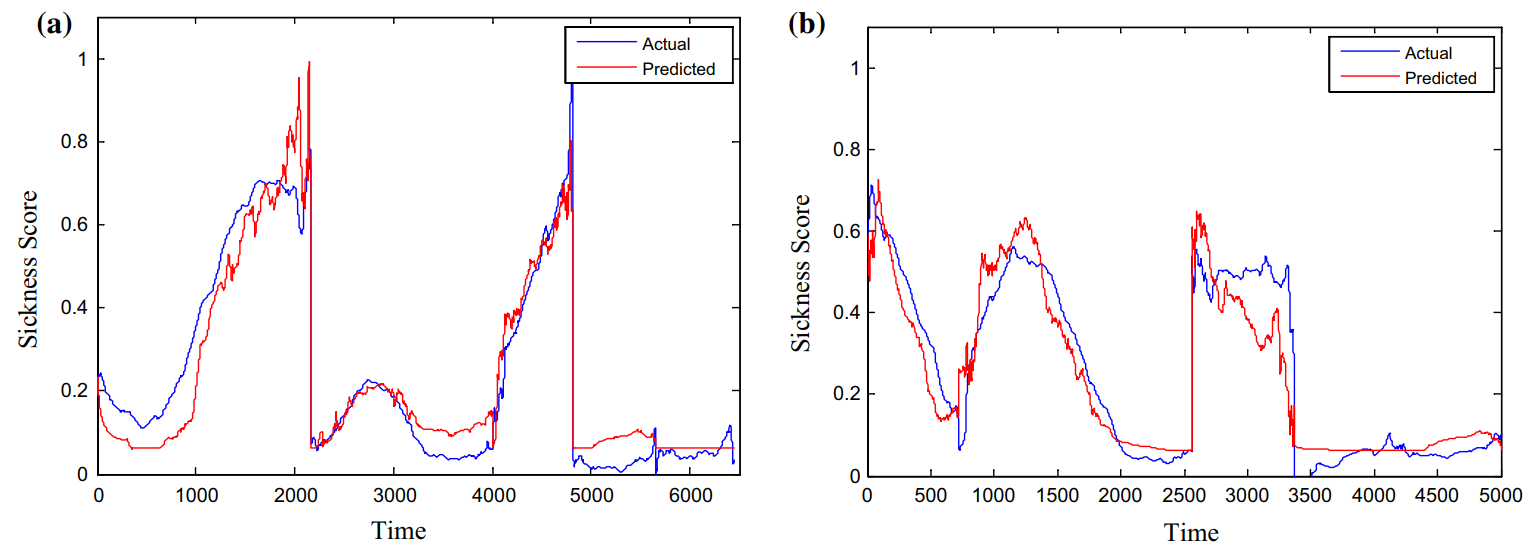
\includegraphics[width=\textwidth]{content/2_related_work/img/PosturalStabilitySicknessPrediction[Lim2020]}
    \caption{Actual sickness (blue) and predicted sickness (red) of (a) training and (b) testing set produced by the
    prediction algorithm by Lim et al.~\cite{Lim2020}.}
    \label{fig:sickness-prediction-algorithm}
\end{figure}
The recent study by Lim et al.~\cite{Lim2020} successfully used postural stability measurements to train an algorithm
to predict VR content's potential to induce cybersickness, as shown in Figure~\ref{fig:sickness-prediction-algorithm},
based on the postural instability theory.


\subsection{Other theories}\label{subsec:other-theories}

\subsubsection{Rest frame theory}
Similar to sensory conflict theory, the rest frame theory argues that a mismatch in sensed gravitation and perceived
up-direction is the cause for sickness symptoms~\cite{Rebenitsch2016}.
\begin{figure}[h]
    \centering
    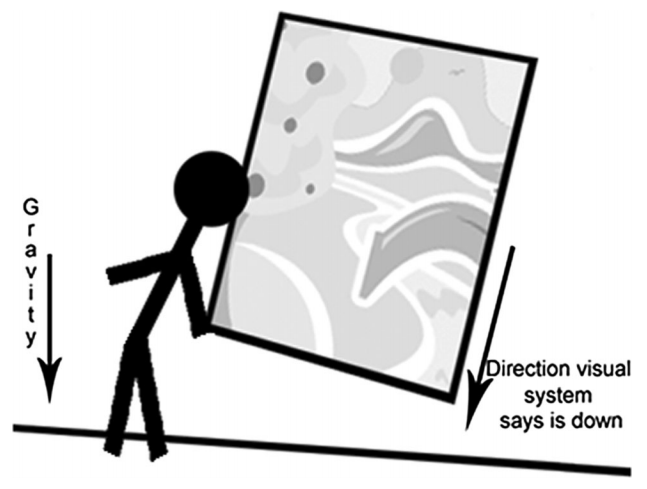
\includegraphics[width=\textwidth/2]{content/2_related_work/img/SensoryMismatchRestFrame[Rebenitsch2016]}
    \caption{Example of sensory mismatch according to rest frame theory~\cite{Rebenitsch2016}.}
    \label{fig:sensory-mismatch-example}
\end{figure}
The rest frame theory also shows similarities to the postural instability theory, as the discrepancy between perceived
up-direction and gravity leads to postural instability and following sickness symptoms~\cite{Rebenitsch2016}.
An example of this sensory mismatch, and resulting postural instability is shown in
Figure~\ref{fig:sensory-mismatch-example}.
The theory also supports the postural instability theory in situations where postural control is lessened, such as in
seated positions where the individual's posture is stabilized.
Several studies like Chang et al.~\cite{Chang2013}, and Duh, Parker, and Furness~\cite{Duh2001b} found, that
superimposing some form of static frame of reference into the virtual environment significantly improves postural
stability and reduces cybersickness symptoms.


\subsubsection{Vergence-accommodation conflict theory}\label{subsubsec:vergence-accommodation-conflict-theory}

Another theory to explain cybersickness symptoms, especially oculomotor symptoms, is the \mbox{vergence-accommodation}
conflict theory.
\begin{figure}[h]
    \centering
    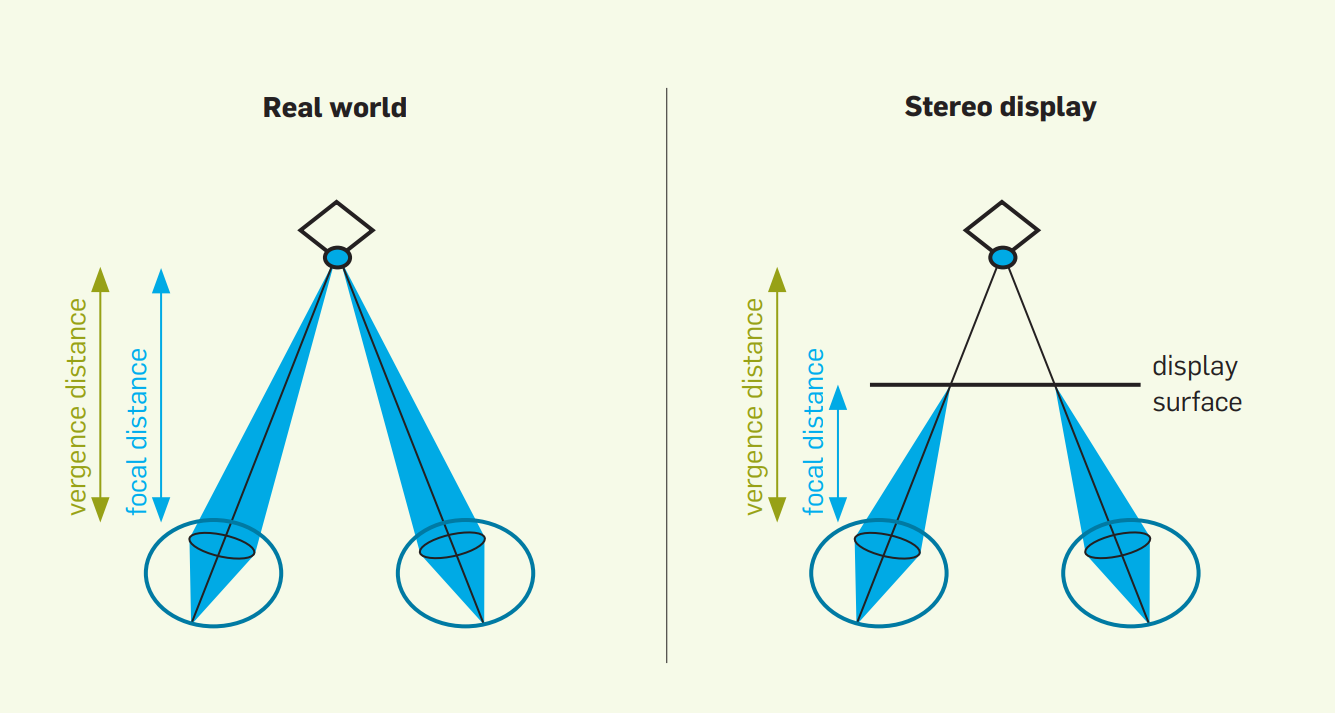
\includegraphics[width=\textwidth/2]{content/2_related_work/img/VergenceAccommodation[Kroeker2010]}
    \caption{Difference between vergence and accomodation distance in the real world (left) and stereoscopic displays
        (right)~\cite{Kroeker2010}.}
    \label{fig:vergence-accommodation-differences}
\end{figure}
Vergence is the simultaneous lateral movement of the eyes when an individual's visual system is adjusting to objects
at different distances~\cite{Kim2014}.
Accommodation is the process of adjusting both eye's focal lengths, focusing on the perceived
object~\cite{Rebenitsch2016}.
In virtual environments, especially in head-mounted displays, images are presented at a fixed screen depth.
This leads to conflict with real life expectations, as vergence and accommodation do not occur naturally at
different distances like in stereoscopic displays~\cite{Saredakis2020}, as shown in
Figure~\ref{fig:vergence-accommodation-differences}.
Kim, Kane, and Banks~\cite{Kim2014} noted that content with high levels of stimulation usually contain more changes
in stimulus distance, and therefore variance of stimulus distance, and level of visual stimulation both increase visual
discomfort and eye strain.


\section{Methods of measurement}\label{sec:methods-of-measurement}

Due to the polysymptomatic and polygenic nature of cybersickness, measurements of cybersickness can prove
difficult, as there is a variety of mostly internal, nonobservable, and subjective symptoms~\cite{McCauley1992}.
Additionally, there can be large individual differences in symptom profiles and susceptibilty, and most symptoms
develop over time and can occur even after the exposure to virtual environments~\cite{McCauley1992}.
Historically, the use of questionnaires is the most popular method of recording occurrences of
cybersickness~\cite{Rebenitsch2016,Saredakis2020}.
The most widely used questionnaire is the Simulator Sickness Questionnaire (SSQ), developed by Kennedy, Lane, Berbaum,
and Lilienthal~\cite{Kennedy1993}.
Recently, several studies have tried refining the SSQ to adapt it for the assessment of virtual reality and
head-mounted displays, resulting in the Virtual Reality Symptom Questionnaire (VRSQ) by Ames, Wolffsohn, and
McBrien~\cite{Ames2005}, and the CyberSickness Questionnaire (CSQ) by Stone III~\cite{Stone2017}.
In addition to the extensive post-session questionnaires, single item questionnaires like the Fast Motion Sickness
Scale (FMS) by Keshavarz and Hecht~\cite{Keshavarz2011} that are polled in regular intervals during the virtual
environment exposure have gained popularity in cybersickness studies.
Because of the subjective nature of questionnaires, these methods of quantifying cybersickness symptoms have been
criticised and several methods of objective measurement have been researched.
Kim et al.~\cite{Kim2005} studied the changes in sixteen different electrophysiological signals and found several
measurements with a significant positive or negative correlation.
However, these measurements require special equipment that may be unavailable or unintuitive, leading to a low
adoption rate among studies related to cybersickness symptoms and detection.
A more easily accessible method of objective measurement has been measuring the postural stability of individuals
exposed to virtual environments and use the changes in the centre of gravity (CoG) as an indicator for cybersickness
symptoms~\cite{Lim2020}.


\subsection{Questionnaires}\label{subsec:questionnaires}

\subsubsection{Simulator Sickness Questionnaire}\label{subsubsec:simulator-sickness-questionnaire}

The Simulator Sickness Questionnaire developed by Kennedy, Lane, Berbaum, and Lilienthal~\cite{Kennedy1993} is,
despite being developed in 1993, still one of the most popular methods to measure cybersickness
symptoms~\cite{Saredakis2020}.
Kennedy et al.~\cite{Kennedy1993} based their developments on the Pensacola Motion Sickness Questionnaire (MSQ),
where they identified several deficiencies that could be improved:
\begin{itemize}
    \item to provide a more valid index of overall simulator sickness severity as distinguished from motion sickness;
    \item to provide subscale scores that are more diagnostic of the locus of simulator sickness in a particular
    simulator for which overall severity was shown to be a problem;
    \item to provide a scoring approach to make monitoring and cumulative tracking relatively straightforward.
\end{itemize}
As part of the last objective, they sought to eliminate the configural approach of the MSQ allowing to automate the
administation and scoring of results.
Additionally, the studies involving the MSQ used differences between post- and pre-exposure scores as their main
indicator, and a pre-exposure checklist where subjects are asked whether they were in other than their "usual state 
of fitness".
Kennedy et al.~\cite{Kennedy1993} removed both, the two-step approach, and the pre-exposure checklist in an effort to
streamline the administration and scoring process, noting that the SSQ is "intended only for application to 
post-exposure symptoms, with the further precondition that a screening of "unhealthy" subjects is required [before exposure]"~\cite[p.
207]{Kennedy1993}.
To tailor the questionnaire to better fit simulator exposure and its sickness symptoms, Kennedy et al
.~\cite{Kennedy1993} eliminated symptoms that might give misleading indication, were selected too infrequently, or
showed no change in frequency or severity.
Additionally, they sorted the remaining symptoms into separate clusters labeled "Oculomotor" (SSQ-O),
"Disorientation" (SSQ-D), and "Nausea" (SSQ-N).
The distinction allowed to apply a subscale to each cluster, reflecting the impact of simulator exposure on a
different "target system" in the subject.
It also simplified the process of determining where and in what way a simulator may cause problematic
symptoms.
\begin{center}
    \begin{tabular}{ l c c c}
        \toprule
        \textbf{ } & \textbf{ } & \textbf{Weight} & \textbf{ } \\
        \textbf{SSQ Symptom} & \textbf{$N$} & \textbf{$O$} & \textbf{$D$} \\
        \midrule
        General discomfort          & 1 & 1 &   \\
        Fatigue                     &   & 1 &   \\
        Headache                    &   & 1 &   \\
        Eyestrain                   &   & 1 &   \\
        Difficulty focusing         &   & 1 & 1 \\
        Increased salivation        & 1 &   &   \\
        Sweating                    & 1 &   &   \\
        Nausea                      & 1 &   & 1 \\
        Difficulty concentrating    & 1 & 1 &   \\
        Fullness of head            &   &   & 1 \\
        Blurred vision              &   & 1 & 1 \\
        Dizzy (eyes open)           &   &   & 1 \\
        Dizzy (eyes closed)         &   &   & 1 \\
        Vertigo                     &   &   & 1 \\
        Stomach awareness           & 1 &   &   \\
        Burping                     & 1 &   &   \\
        \\
        Total                       & [1] & [2] & [3] \\
        \\
        Score & & & \\
        $N = [1] \times 9.54$ & & & \\
        $O = [2] \times 7.58$ & & & \\
        $D = [3] \times 13.92$ & & & \\
        $TS = [1] + [2] + [3] \times 3.74$ & & & \\
        \bottomrule
    \end{tabular}
    \captionof{table}{SSQ Symptoms and Scoring according to Kennedy et al.~\cite{Kennedy1993}.}
    \label{tab:ssq-scoring}
\end{center}
Table~\ref{tab:ssq-scoring} shows the remaining symptoms and their clustering, as well as the method of scoring the
SSQ as derived by Kennedy et al.~\cite{Kennedy1993}.
The SSQ symptoms are rated on a four-point scale from 0 to 3, then multiplied by either 1 or 0 (omitted in the table)
according to the weight section of table~\ref{tab:ssq-scoring}, and finally summed up in each column.
The total and subscale scores are then calculated using the formulas in the "Score" section of
table~\ref{tab:ssq-scoring}.
Kennedy et al.~\cite{Kennedy1993} also mention the possibility to further refine the questionnaire by:
\begin{itemize}
    \item splitting the "Oculomotor" cluster into the disturbance of visual processing (blurred vision, difficulty
    focusing) and the symptoms caused by the disturbance (headache, eyestrain);
    \item splitting the "Nausea" cluster into premonitory signs (increased salivation, burping) and advanced stages
    of nausea (nausea, sweating);
\end{itemize}
As well as moving some symptoms into a "tired and hungry" cluster, believed to be an artifact created by the time
spent during the exposure.
However, Kennedy et al.~\cite{Kennedy1993} state that there are not enough simulator-relevant symptoms to provide
adequate reliability for smaller clusters, and recommend using the three cluster solution.
Despite the general adoption of the SSQ, there are several problems, especially for the assessment of
cybersickness symptoms in virtual environments, that Kennedy et al.~\cite{Kennedy1993} recognize in their study.
\begin{center}
    \begin{tabular}{ l l c c c c}
        \toprule
         & & & \textbf{SSQ} & \textbf{Scale M} & \\
        \textbf{Simulator} & \textbf{Aircraft} & \textbf{$N$} & \textbf{$O$} & \textbf{$D$} & \textbf{$TS$*} \\
        \midrule
        2F64C & SH-3   & 14.7 & 20.0 & 12.4 & 18.8 \\
        2F120 & CH-53E & 7.5  & 10.5 & 7.4  & 10.0 \\
        2F121 & CH-53D & 7.2  & 7.2  & 4.0  & 7.5  \\
        2F110 & E-2C   & 7.1  & 13.1 & 6.8  & 10.3 \\
        2E7   & F/A-18 & 6.1  & 5.1  & 6.2  & 6.8  \\
        2F117 & CH-46E & 5.4  & 7.8  & 4.5  & 7.0  \\
        2F87F & P-3C   & 4.5  & 15.2 & 4.3  & 10.5 \\
        2F132 & F/A-18 & 2.7  & 6.1  & 0.6  & 4.2  \\
        2F112 & F-14   & 1.7  & 1.8  & 0.0  & 1.5  \\
              &        &      &      &      &      \\
        M     &        & 7.7  & 10.6 & 6.4  & 9.8  \\
        SD    &        & 15.0 & 15.0 & 15.0 & 15.0 \\
        \bottomrule
        * Total Severity & & & & & \\
    \end{tabular}
    \captionof{table}{SSQ Scale Means by Simulator for the Calibration Sample according to Kennedy et al
    .~\cite{Kennedy1993}.}
    \label{tab:ssq-calibration}
\end{center}
The weights for the scoring functions are derived from 1119 pairs of MSQs collected from 9 simulator sites
shown in table~\ref{tab:ssq-calibration} as a calibration sample.
Therefore, the modal position on the Symptoms or the intermediate sums is no indication for symptomatology with
respect to simulator sickness across simulators in general, as the zero point contains between 40\% and 75\% of the
observations in the calibration dataset.
This also means, the sensitivity is at the upper extremes of the symptomatology range, and the scores should be
compared to the calibration set, in table~\ref{tab:ssq-calibration}, instead of
interpreted on their own~\cite{Kennedy1993}.
Kennedy et al.~\cite{Kennedy1993} conclude that the results should not be used to distinguish among simulators without
problems, but identify and discriminate problem simulators from those without problems.
Other, more recent studies, like Sevinc and Berkman~\cite{Sevinc2020}, and Rebenitsch and Owen~\cite{Rebenitsch2016},
criticise the usage of the Simulator Sickness Questionnaire because of its complex structure, and development
process, as it involves only a sample of highly trained professionals, and a small amount of simulator experiments,
which both do not comply with the modern day HMD-based virtual environments, and diverse applications
and users~\cite{Sevinc2020}.

\subsubsection{Virtual Reality Symptom Questionnaire}

Recent studies like Ames, Wolffsohn, and McBrien~\cite{Ames2005} tried to develop a questionnaire based on the MSQ
and SSQ specifically for the assessment of cybersickness symptoms.
Ames et al.~\cite{Ames2005} note that existing methods like the SSQ do not properly address the ocular symptoms that
contribute to cybersickness symptoms in virtual environments.
Examining existing virtual reality research, they identified 23 symptoms split into two clusters, 12 non-ocular, and
11 ocular symptoms.
Ames et al.~\cite{Ames2005} also decided to expand the symptom response scale to seven options sorted into four
labels: "none" (0), "slight" (1, 2), "moderate" (3, 4), and "severe" (5, 6).
In the development study, they exposed 16 subjects to a stereoscopic video played on a
head-mounted display, and recorded the occurring symptoms with the developed VRSQ in two-minute
intervals immediately after the exposure for a total of six post-exposure examinations.
From the results, they identified 13 symptoms with high item-total correlations, that remain in the final
questionnaire.
While, the "nausea" symptom did not meet the correlation criteria, it was retained for research that might involve
more "dynamic imagery".
However, similar studies, like Stone III~\cite{Stone2017}, criticise the validity of the VRSQ to evaluate
cybersickness, as Ames et al.~\cite{Ames2005} only used video input on a head-mounded display, without any user
interaction or input method, resulting in visual stimulus only, similar to existing studies on visually induced motion
sickness, but not explicitly virtual reality sickness symptoms.
Additionally, Stone III~\cite{Stone2017} notes concerns about the validity of the psychometric evaluation, and the
small sample size used in the development study.
Davis, Nesbitt, and Nalivaiko~\cite{Davis2014} also note the lack of published studies using the VRSQ as a method to
evaluate cybersickness symptoms in their review on cybersickness literature, while Rebenitsch et al
.~\cite{Rebenitsch2016} do not mention the VRSQ at all.

\subsubsection{CyberSickness Questionnaire}

In his study criticising the VRSQ and SSQ, Stone III~\cite{Stone2017} also proposes an alternative solution to
measure cybersickness symptoms, the CyberSickness Questionnaire (CSQ).
Similar to the method Kennedy et al.~\cite{Kennedy1993} used to refine the SSQ from the MSQ, they reinterpreted the
results of the SSQ in a cybersickness context.
For this, Stone III~\cite{Stone2017} selected the symptoms clearly indicating cybersickness:
\begin{itemize}
    \item headache
    \item eyestrain
    \item nausea
    \item blurred vision
    \item dizzy (eyes open)
    \item dizzy (eyes closed)
    \item vertigo
    \item difficulty focusing
    \item fullness of head
\end{itemize}
Additionally, they decided to amalgamate "Severe" and "Moderate" responses from the SSQ.
Stone III~\cite{Stone2017} found a two factor solution by separating the Symptoms into two clusters: "Dizziness" and
"Difficulty focusing".
They also note that the SSQ can still be used to record post-exposure symptoms, while the
scoring can be done using the developed CSQ approach by following these steps:
\begin{enumerate}
    \item Administer the SSQ after the exposure to virtual environments.
    \item Remove the unneccesary symptom items from the collected data.
    \item Combine "Moderate" and "Severe" options for each symptom item, resulting in responses "None" (0), "Slight"
    (1), and "Moderate" (2).
    \item Compute the CSQ factors, similar to the SSQ, by multiplying each symptom item with the weight shown in
    table~\ref{tab:csq-scoring} and adding up the items to form the final scores.
\end{enumerate}
\begin{center}
    \begin{tabular}{ l l l}
        \toprule
        \textbf{} & \textbf{Dizziness} & \textbf{Difficulty focusing} \\
        \midrule
        Headache                & $.50$ & $.$   \\
        Eyestrain               & $.$   & $.58$ \\
        Difficulty focusing     & $.$   & $.89$ \\
        Nausea                  & $.84$ & $.$   \\
        Fullness of head        & $.$   & $.55$ \\
        Blurred vision          & $.$   & $.81$ \\
        Dizziness (eyes open)   & $.89$ & $.$   \\
        Dizziness (eyes closed) & $.99$ & $.$   \\
        Vertigo                 & $.54$ & $.$   \\
        \bottomrule
    \end{tabular}
    \captionof{table}{CSQ nine-item, two-factor model for scoring, according to Stone III~\cite{Stone2017}}
    \label{tab:csq-scoring}
\end{center}
Stone III~\cite{Stone2017} notes that preliminary evidence, and the comparison of CSQ scores with other established
visually-induced motion sickness scoring methods support the validity of the resulting CyberSickness Questionnaire.
However, they note based on the CSQ scores of their study, 57\% of the 202 participants reported no dizziness and 40\%
reported no difficulty focusing, which implies cybersickness was very low, and the study was not focused
explicitly on inducing cybersickness symptoms.
The review of questionnaires by Sevinc et al.~\cite{Sevinc2020} has tested and approved the validity of the CSQ and
concludes that it is a more accurate method of measuring cybersickness symptoms than the SSQ, as it was developed
with a lager sample size and specifically based on the use of virtual reality applications to induce sickness symptoms.
